\documentclass[a4paper, 1.5lines]{ctexart}
\usepackage[top=3cm, bottom=2cm]{geometry}
\usepackage{graphicx}
\usepackage{subcaption}
\usepackage{amsmath}
\usepackage{amssymb}
\usepackage{xcolor}
\usepackage{url}
\usepackage{booktabs}
\usepackage{multirow}
%\usepackage{hyperref}
\usepackage[hidelinks]{hyperref} % 加载 hyperref 并隐藏链接边框

%\usepackage[utf8]{inputenc}
%\usepackage[ngerman]{babel} % 加载德语支持

% booktabs 提供 \toprule, \midrule, \bottomrule 等表格命令
\usepackage{booktabs}
% 定义占位命令以避免未定义控制序列错误
\newcommand{\placeholderspace}{}
\usepackage{fancyhdr} % 导入fancyhdr宏包
\usepackage{lipsum}   % 仅用于生成示例文本
\usepackage{float}    % 提供 H 浮动位置选项

% 设置页面样式为fancy
\pagestyle{fancy}
% 自定义页眉内容
\fancyhead[L]{} % 左侧页眉
\fancyhead[C]{\textbf{Physics-experiment Reporting Letter:\\Microwave and Ferromagnetic Resonance}} % 中间页眉
\fancyhead[R]{ } % 右侧页眉
% 自定义页脚内容
\fancyfoot[L]{ } % 左侧页脚
\fancyfoot[C]{\thepage} % 中间页脚显示页码
\fancyfoot[R]{ } % 右侧页脚
% 改变页眉线的粗细
\renewcommand{\headrulewidth}{1.4pt}
% 改变页脚线的粗细
\renewcommand{\footrulewidth}{0.pt}





\title{微波与铁磁共振}
\author{实验人：学生\qquad 学号：[学号已脱敏]\qquad 指导教师：张耀峰}
\date{实验日期：2026.3.6}


\begin{document}
    
    \maketitle
    
    \begin{abstract}
         
        本实验利用体效应振荡管产生微波并研究其基本性质，同时结合谐振腔系统探究单晶与多晶样品的磁共振特性。首先通过测量振荡管的 I-U 曲线验证其负阻特性，从而说明微波产生的物理机制。随后在波导系统中测量微波功率与频率之间的关系，并绘制相应曲线。接着利用谐振腔测量谐振频率，并与理论结果进行比较，以验证谐振腔的电磁模式特性。在外加磁场作用下，样品满足共振条件 $h\nu = g\mu_B B$ 时产生磁共振吸收现象，通过比较单晶与多晶样品的共振曲线，可以观察到谱线形状和宽度上的差异。最后通过逐点法测量多晶样品的磁共振曲线，并结合磁场测量结果计算得到朗德因子 $g = 2.045$ 和弛豫时间 $\tau = 1.65 \times 10^{-10}\,s$。

        \textbf{\textbf{关键词：微波\quad 铁磁共振\quad 谐振腔\quad 体效应振荡管}}
    \end{abstract}
    
    \section{引言}
        微波是电磁波谱中的重要组成部分，在通信、雷达和材料研究等领域具有广泛应用。铁磁共振则是研究物质内部磁相互作用的重要实验方法，通过观测材料在射频磁场和外加静磁场共同作用下的共振吸收现象，可以获得材料的磁学参数及其微观动力学特性。因此，研究微波产生与铁磁共振现象，对于理解电磁波与物质相互作用具有重要意义。

        本实验利用砷化镓（GaAs）体效应振荡管产生稳定的微波信号，并通过测量振荡管的 I-U 特性验证其负阻特性，从而理解微波振荡产生的物理机制。在此基础上，通过波导系统研究微波的传播特性，并利用传输式谐振腔研究样品在射频磁场中的共振行为。

        实验中分别对单晶和多晶样品进行磁共振测量，通过比较其共振曲线的形状与宽度，分析不同晶体结构对磁共振特性的影响。通过实验数据还可以进一步计算旋磁比、朗德因子 $g$ 以及弛豫时间 $\tau$ 等重要物理参数，从而加深对电子自旋共振及其相关物理过程的理解。
    \section{原理}

    \subsection{微波的产生}

微波为波长 $\lambda \in (0.1\,\text{cm},\,100\,\text{cm})$ 范围内的电磁波。微波具有高频性、短波性、似光性以及量子性等特点。

通常利用以 GaAs 为材料制作的微波体效应振荡器产生微波振荡。GaAs 的能带结构中具有多个能谷，其中最重要的是位于布里渊区中心、能量最低的主能谷（低能谷）以及其邻近的高能谷。由于这种多能谷结构，使得 GaAs 在一定电压范围内会出现电子迁移率下降，从而表现出负阻效应。

由于晶体管阴极附近存在较大的接触电阻以及杂质分布不均匀，这种不均匀性会形成局部的偏极化区域并产生高场畴。高场畴的形成与移动会使 GaAs 的电流特性曲线出现陡降和回滞区，从而形成明显的负阻区域。电流增大过程中高场畴形成的阈值电压记为 $V_{\text{th}}$。

当器件的偏压 $V_b > V_{\text{th}}$ 时，设交流电压振幅为 $V_{\text{ac}}$，器件两端的总电压为
\begin{equation}
V(t) = V_b + V_{\text{ac}}\cos(\omega_0 t)
\end{equation}

此时体效应管在负阻区工作，从而能够产生稳定的微波振荡。

\subsection{微波的传输与测量}

\subsubsection{传输——波导管}

本实验中波导主要传播 $TE_{10}$ 模式，相应的电磁场分布为

\begin{align}
E_x &= 0, &
H_x &= -\frac{\beta}{\omega\mu}E_0 \sin\left(\frac{\pi x}{a}\right)\exp[i(\omega t-\beta z)] \\
E_y &= E_0 \sin\left(\frac{\pi x}{a}\right)\exp[i(\omega t-\beta z)], &
H_y &= 0 \\
E_z &= 0, &
H_z &= \frac{\omega\mu a}{i\pi}E_0 \cos\left(\frac{\pi x}{a}\right)\exp[i(\omega t-\beta z)]
\end{align}

其中 $a$ 为波导的宽边长度。对于 $TE_{10}$ 模式，其截止波长为

\begin{equation}
\lambda_c = 2a
\end{equation}

波导波长为

\begin{equation}
\lambda_g = \frac{\lambda}{\sqrt{1-\left(\frac{\lambda}{\lambda_c}\right)^2}}
\end{equation}

\subsubsection{微波测量}

\begin{enumerate}

\item 频率测量——谐振腔法：  
利用共振吸收原理，当频率计谐振频率与微波频率相同时会发生强烈吸收，通过查表即可得到微波频率。

\item 功率测量——晶体检波器：  
采用相对测量方法，在晶体检波器与波导调谐达到最大信号时，有
$I = \text{Const}\cdot P$，
通过测量电流即可表征对应的微波功率。

\end{enumerate}

\subsection{铁磁共振原理}

当射频磁场频率 $\omega$ 满足

\begin{equation}
\omega = \omega_0 = \gamma B_0
\end{equation}

时发生铁磁共振。其中 $\gamma$ 为旋磁比：

\begin{equation}
\gamma = g\frac{e}{2m}
\end{equation}

铁磁体的磁导率张量可表示为

\begin{equation}
\mu =
\begin{pmatrix}
\mu - i\kappa & i\kappa & 0 \\
- i\kappa & \mu - i\kappa & 0 \\
0 & 0 & \mu_z
\end{pmatrix}
\end{equation}

其中  
$\mu = \mu' - i\mu''$，  
$\kappa = \kappa' - i\kappa''$，  
$\mu_z = \mu'_z - i\mu''_z$。

在实验中保持射频磁场不变，改变外加稳恒磁场 $H$ 的大小，可以得到 $\mu''$ 随 $H$ 的变化曲线，该曲线称为铁磁共振曲线。其形状表现为对称型吸收峰，半高宽记为 $\Delta H$。由此可以得到弛豫时间

\begin{equation}
\tau = \frac{2}{\gamma \Delta B}
\end{equation}

\subsection{谐振腔}

谐振条件为

\begin{equation}
l = p\lambda_g , \quad p\in\mathbb{N}
\end{equation}

谐振曲线的有载品质因数为

\begin{equation}
Q_L = \frac{f_0}{|f_1 - f_2|}
\end{equation}

其中 $f_0$ 为谐振频率，$|f_1-f_2|$ 为传输系数曲线 $T(f)-f$ 的半高宽。

\subsection{测量原理}

根据微扰理论，将样品放入谐振腔后会引起谐振频率和品质因数的变化，其修正关系为

\begin{equation}
\frac{f-f_0}{f_0} = -A(\mu'-1), \qquad
\Delta\left(\frac{1}{Q_L}\right) = 2A\mu''
\end{equation}

    \section{实验}

    \subsection{实验仪器}

\begin{itemize}

\item \textbf{微波体效应振荡器}

微波体效应振荡器用于产生稳定的微波信号，是本实验的主要微波源。该装置基于 GaAs 体效应管的负阻特性，在适当偏置电压下能够产生稳定的微波振荡。本实验中其工作电压范围一般为 $10\sim13\,\text{V}$。

\item \textbf{微波测量仪器}

实验中采用吸收式频率计测量微波频率，晶体检波器用于检测微波功率，测量线用于观察和调整波导系统的驻波情况。这些仪器共同构成微波参数测量系统。

\item \textbf{传输式谐振腔}

传输式谐振腔用于产生稳定的射频磁场并观察铁磁共振现象。该装置由带耦合孔的矩形波导构成，在特定频率下能够形成驻波并增强微波场强，从而便于研究样品在微波作用下的磁共振特性。

\end{itemize}


\subsection{实验内容}

\subsubsection{微波体效应振荡器工作曲线及性能测量}

\begin{enumerate}

\item 打开体效应微波振荡器，调节“频率”旋钮使频率约为 $9.000\,\text{GHz}$，并保证电源预热约 $30\,\text{min}$。

\item 按下“等幅”和“教学”工作按钮，在 $0\sim13\,\text{V}$ 范围内连续改变体效应管的工作电压，记录对应的工作电流，绘制体效应管的 $I-U$ 特性曲线。同时利用吸收式频率计和检波器测量 $10\sim13\,\text{V}$ 区间内频率随电压变化的关系曲线，分析体效应管的负阻区及微波工作区电压范围。

\item 将体效应管工作电压调至标准值（约 $12.0\,\text{V}$），调节功率控制旋钮和微波衰减器，使检波器1连接的微安表指示合适。改变微波频率（$8.9\sim9.2\,\text{GHz}$），记录不同频率下的微波输出功率，并在每次调节频率后重新调谐检波器。

\end{enumerate}


\subsubsection{铁磁共振实验}

\begin{enumerate}

\item 检查传输式谐振腔内金属耦合片是否正确安装。

\item 根据参数 $p=8$，$a=2.295\,\text{cm}$，$l=19.30\,\text{cm}$ 估算谐振腔理论谐振频率：
\[
l=p\cdot\frac{\lambda_g}{2}, \qquad
\lambda_g=\frac{\lambda}{\sqrt{1-(\lambda/\lambda_0)^2}}, \qquad
\lambda_0=2a, \qquad
\lambda=\frac{c}{f}.
\]

\item 将电磁铁电流调至最小，打开共振仪电源并设为检波模式。在理论谐振频率附近调节微波频率，当检波指示发生变化时，调节检波器2的调谐活塞及灵敏度。

\item 细调微波频率以确定谐振腔的最佳谐振频率 $f_0$。连接微安电流表并调节衰减器，使电流表示数合适。以 $f_0$ 为中心逐点测量谐振曲线，并计算品质因数 $Q_L$。

\item 将微波频率固定在 $f_0$，切换至扫场模式，放入铁氧体样品。逐渐增大磁场电流，在示波器（X-Y 模式）上观察共振曲线，并通过调节相移旋钮优化曲线形态。

\item 更换不同类型样品（如单晶或多晶），观察其共振信号变化并记录共振曲线。

\item 采用逐点法测量共振线宽 $\Delta H$：保持谐振腔最佳调谐状态，在检波模式下逐渐改变磁场电流，记录共振曲线数据。

\item 使用高斯计测量电磁铁电流与磁场强度之间的关系，并据此计算旋磁比 $\gamma$（满足 $\omega_0=\gamma B_0$）、$g$ 因子以及弛豫时间 $\tau$。

\item 分析不同样品弛豫时间差异的可能原因。

\end{enumerate}

    \section{结果与分析结论}

    \subsection{体效应振荡器工作曲线测量及性能测量}

\subsubsection{体效应管 $I-U$ 曲线}

在 $0\sim13\,\text{V}$ 的电压范围内测量体效应管的 $I-U$ 特性曲线，并分别记录升压与降压过程的数据，得到结果如图\ref{fig:IU} 所示。

\begin{itemize}

\item \textit{升压过程}

在升压过程中，当 $U < 2.5\,\text{V}$ 时，电流随电压增加迅速增大，表现为正常的正阻特性。当电压接近 $U \approx 2.7\sim2.9\,\text{V}$ 时，电流达到最大值，约为 $I \approx 420\,\text{mA}$。继续增加电压后，电流反而开始减小，曲线出现明显的负斜率区间，表明体效应管进入负阻区。该现象说明器件内部形成并传播高场畴，这是体效应振荡产生微波的物理基础。

在 $3\sim8\,\text{V}$ 的电压范围内，电流总体呈缓慢下降趋势，体现出稳定的负阻特性。当电压进一步增大至 $8\,\text{V}$ 以上时，电流变化逐渐趋于平缓，并在较高电压区域保持在约 $290\sim300\,\text{mA}$ 附近。

\item \textit{降压过程}

在降压过程中测得的曲线与升压过程整体趋势基本一致，两条曲线几乎重合，仅在部分电压区域存在轻微偏差。这种差异表明器件在高场畴形成与消失过程中存在一定的迟滞效应，但整体迟滞现象较弱。

\end{itemize}

\begin{figure}[h!]
\centering
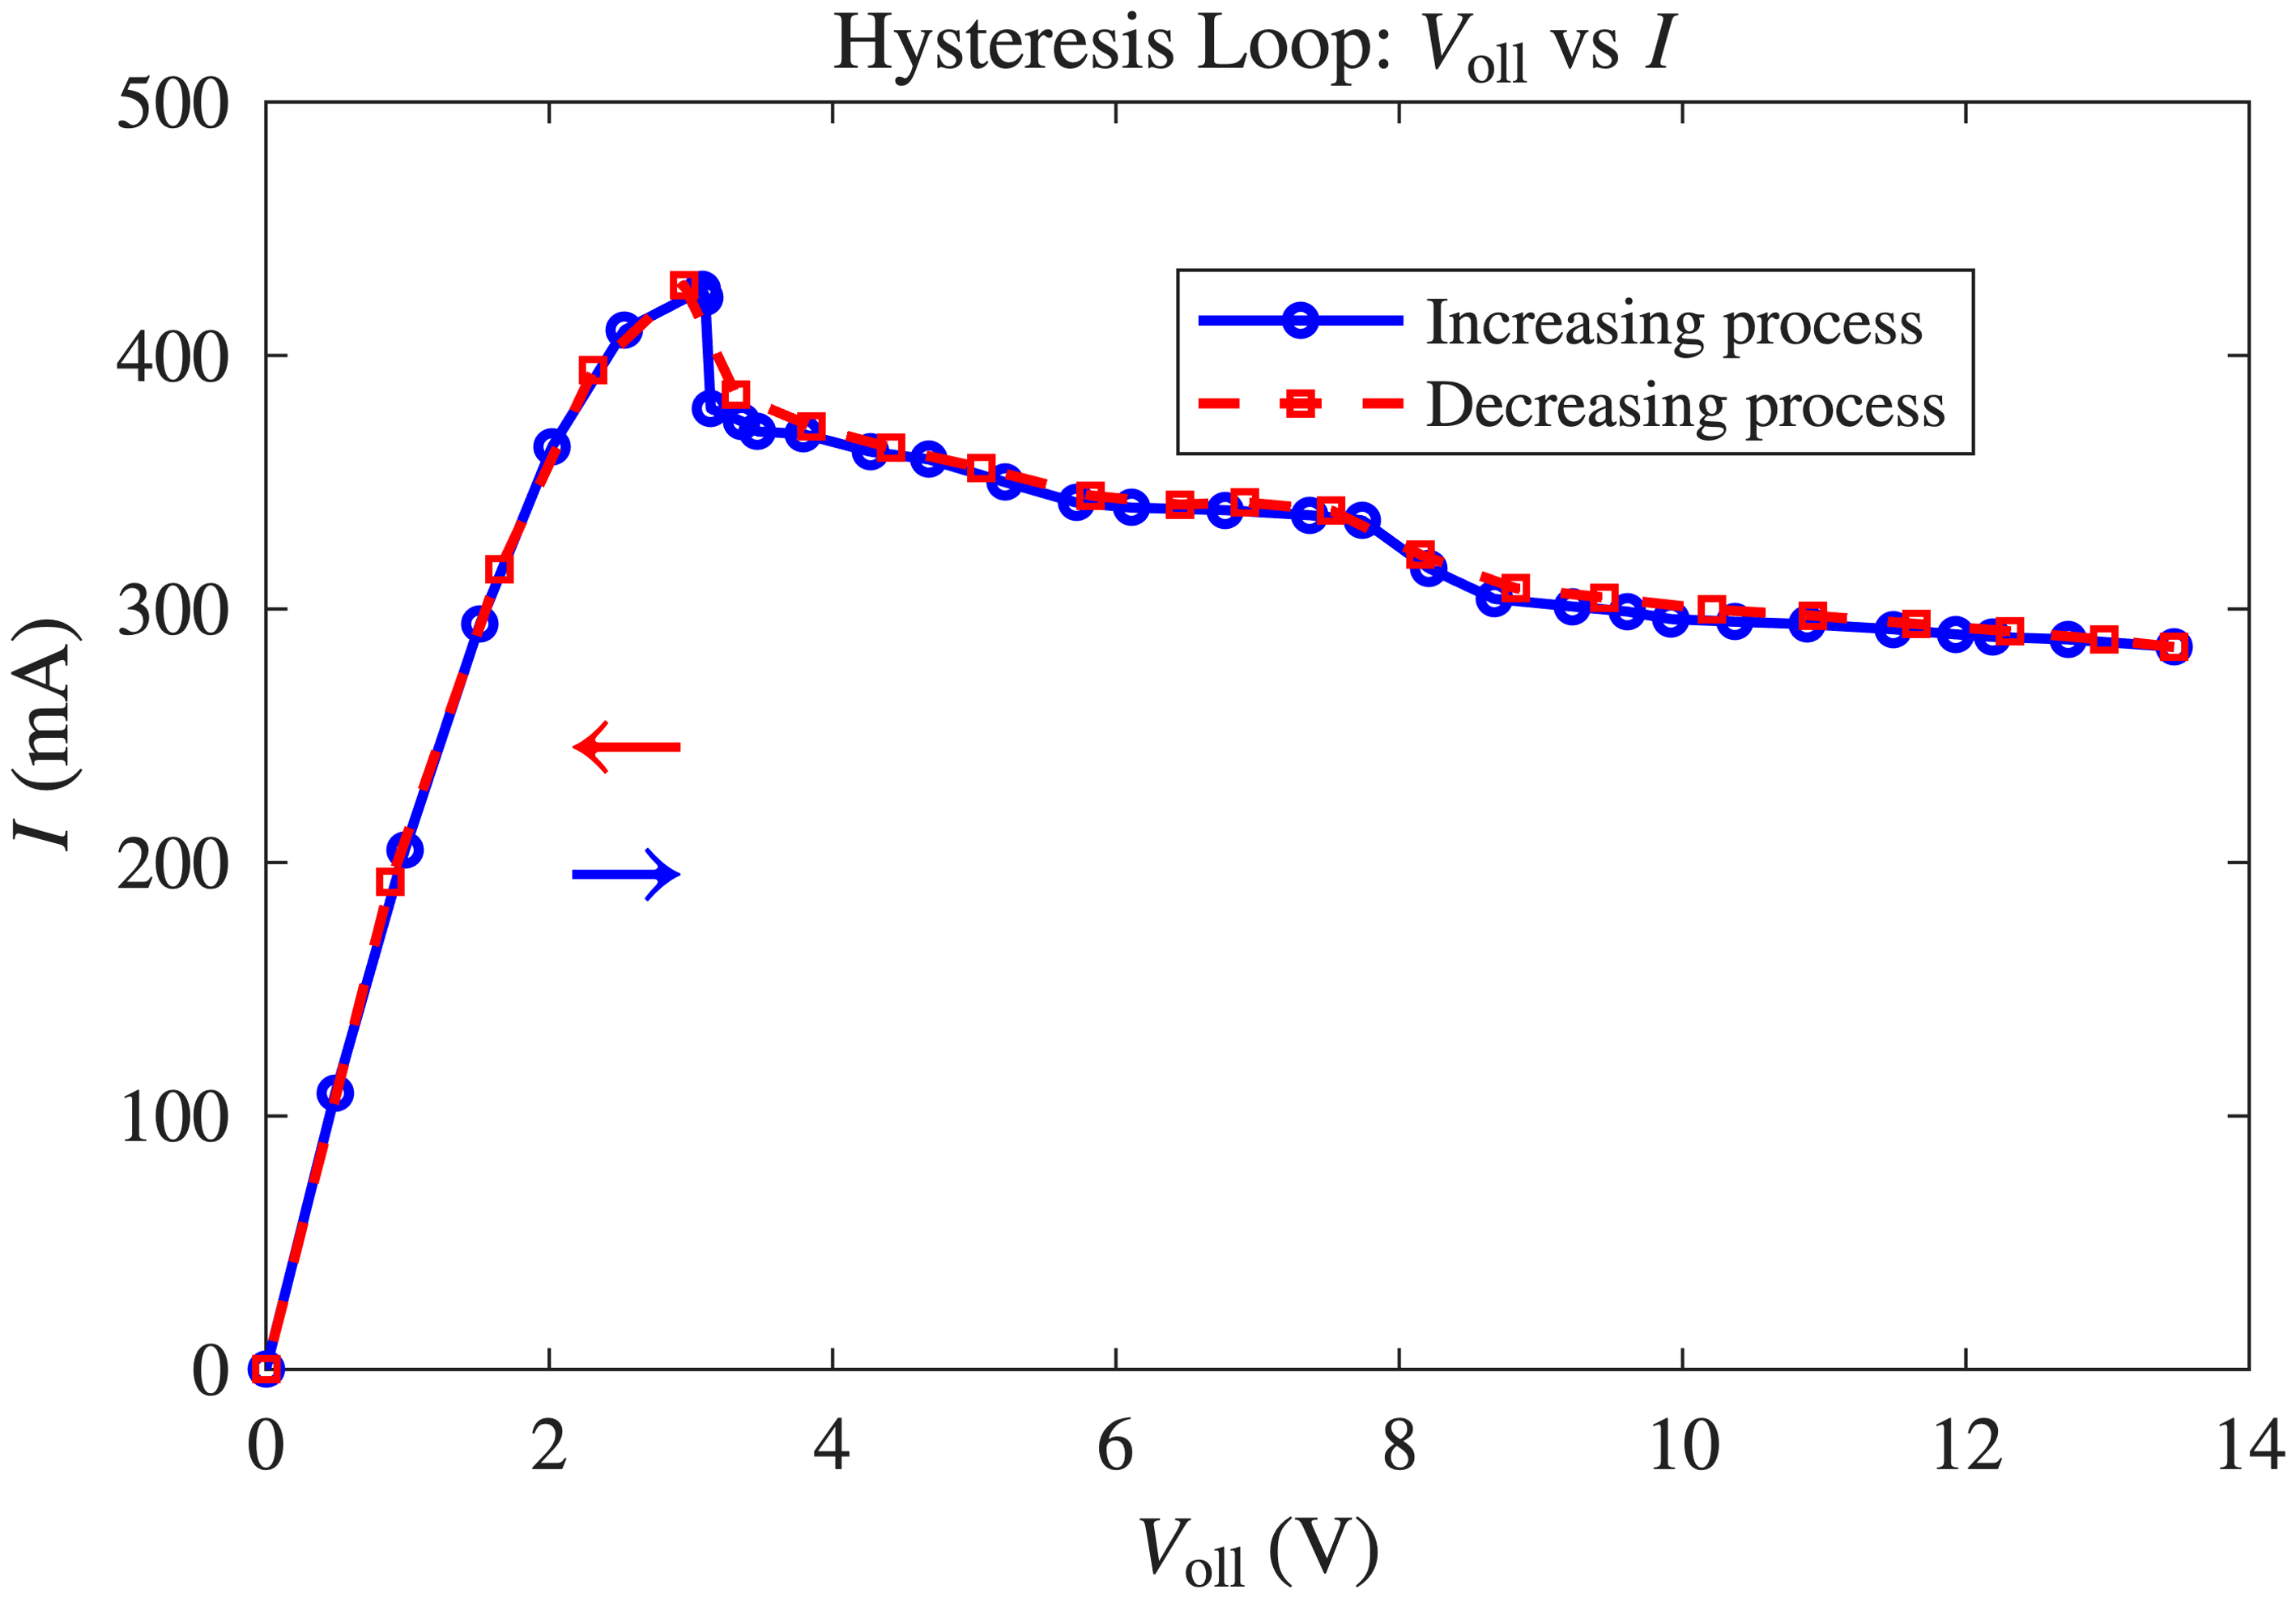
\includegraphics[width=\textwidth]{fig/fig1.png}
\caption{体效应管 $I-U$ 曲线}
\label{fig:IU}
\end{figure}

综合实验结果可以看出，体效应管在约 $2.8\,\text{V}$ 附近出现电流峰值并进入负阻区，该负阻区正是体效应振荡器能够产生微波振荡的工作区间。

\begin{figure}[h!]
\centering
\begin{subfigure}{0.46\textwidth}
\centering
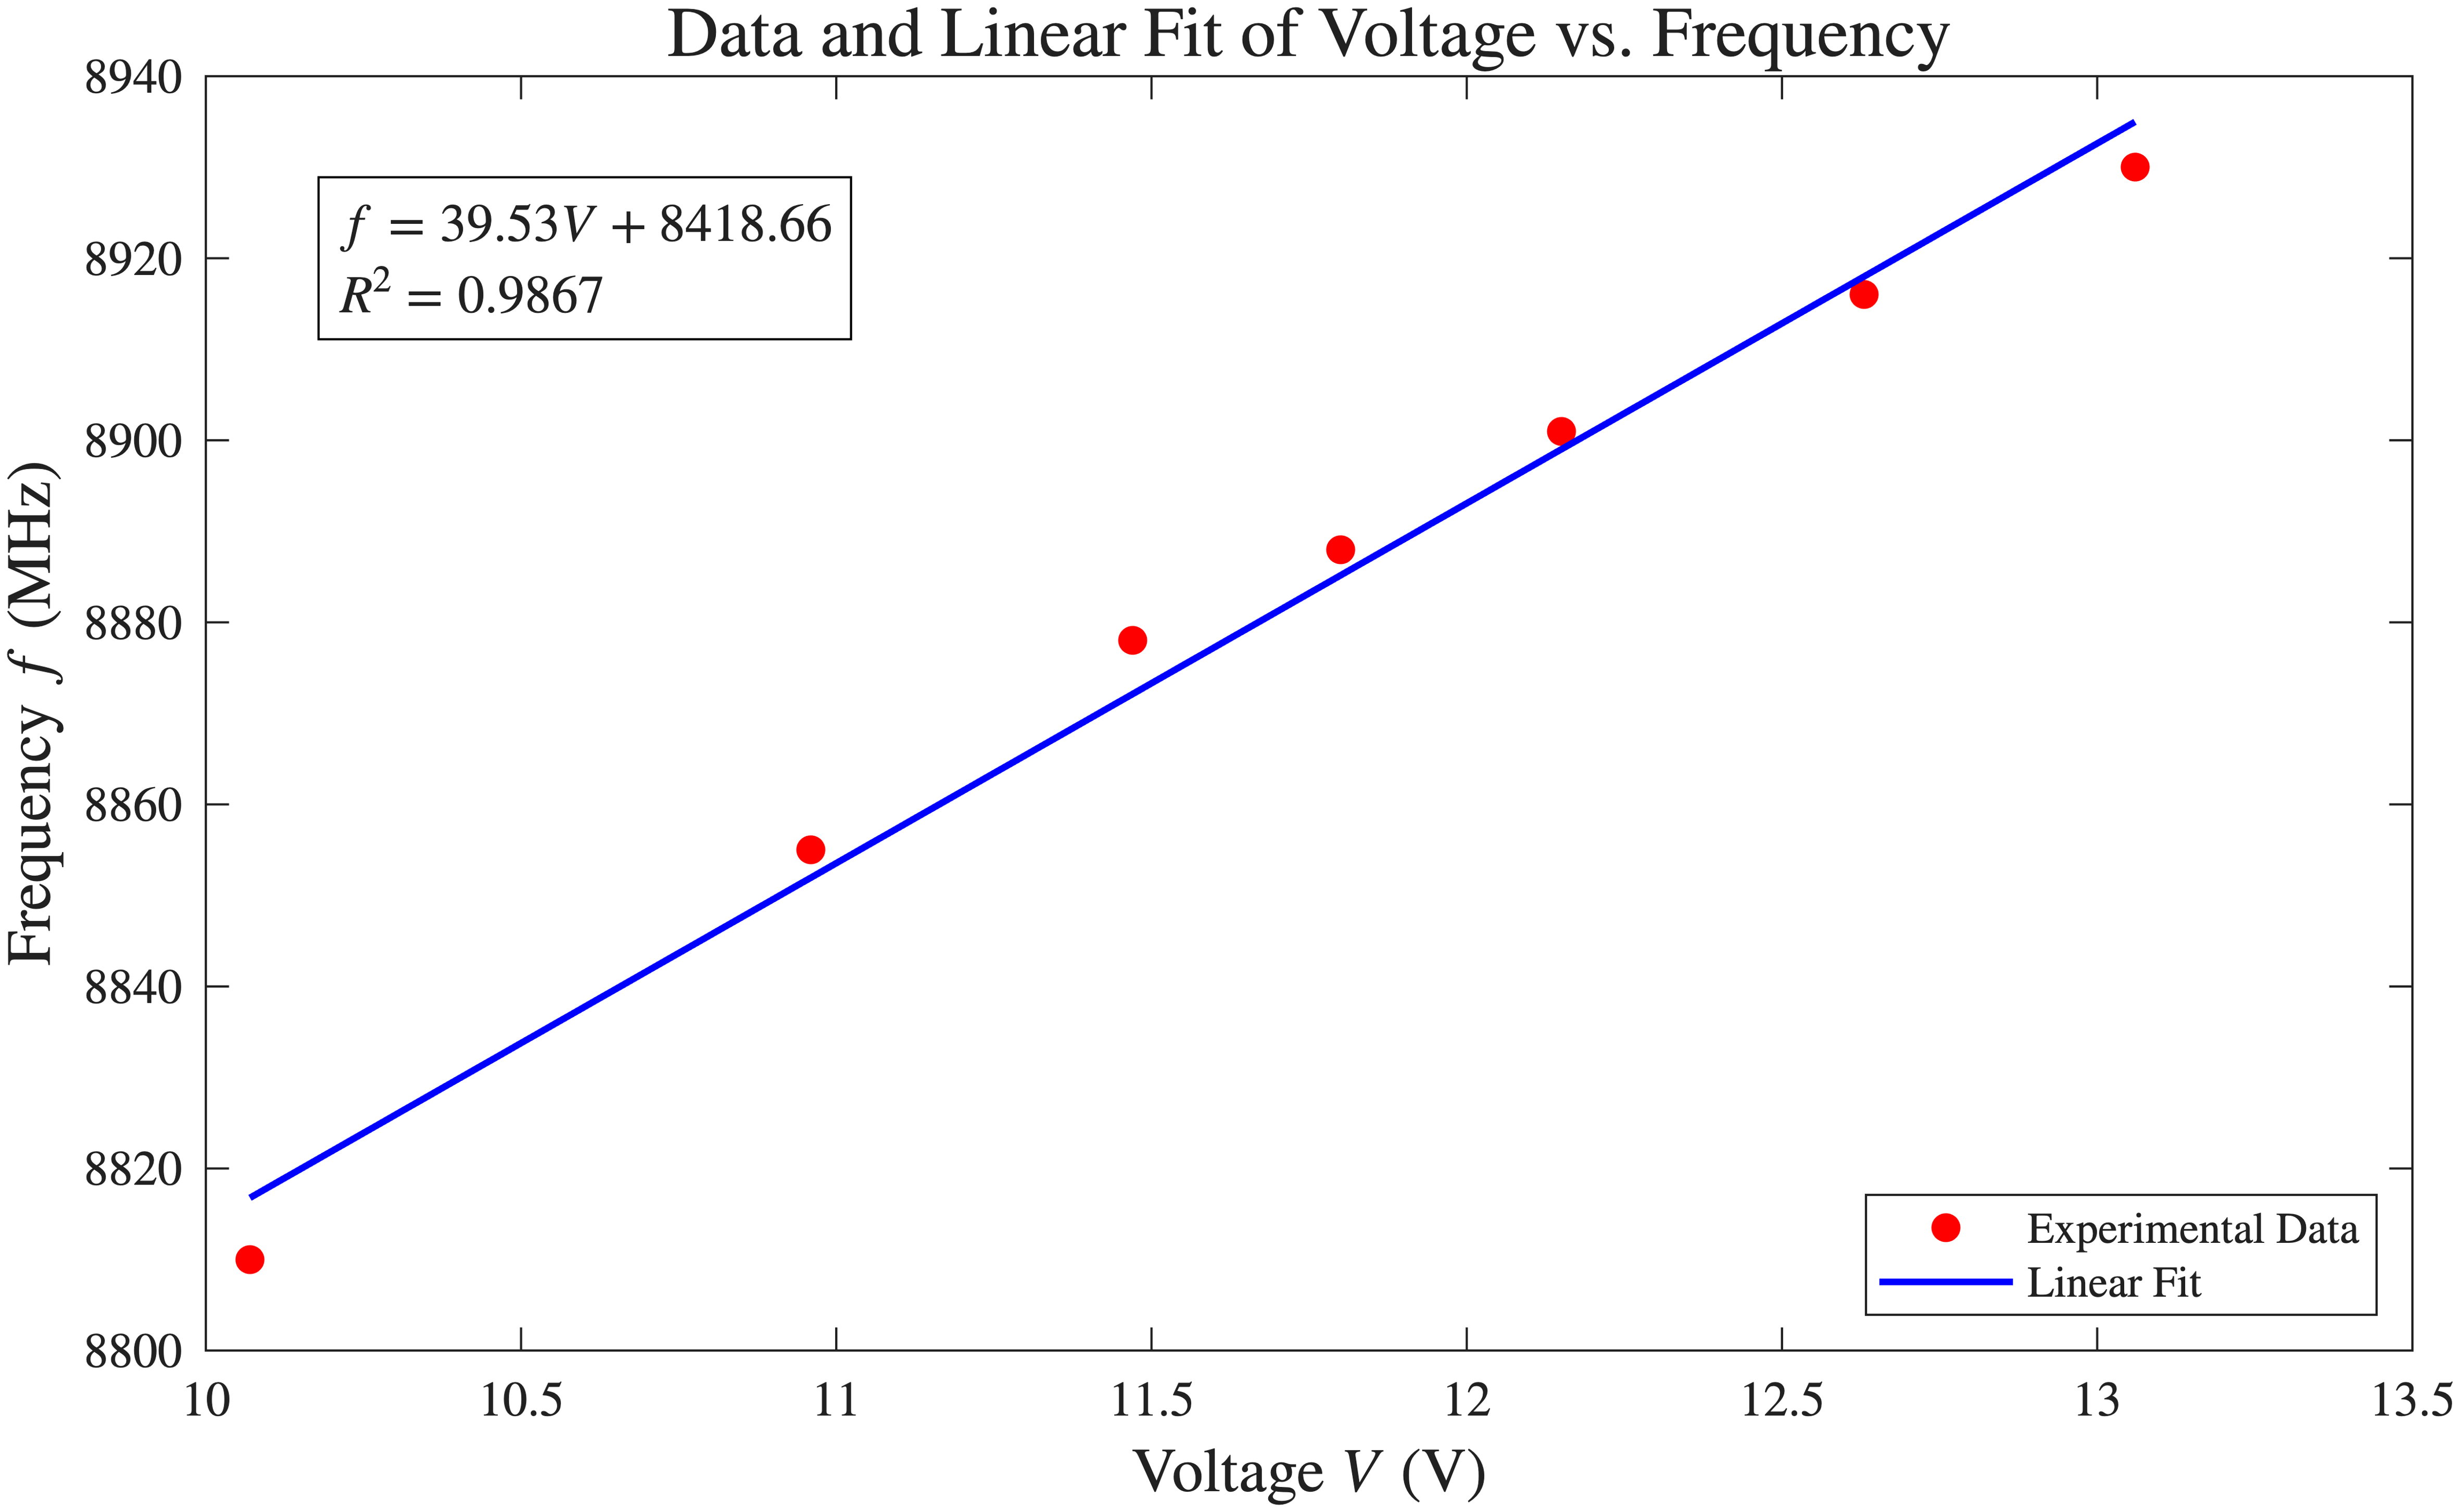
\includegraphics[width=\textwidth]{fig/fig2.png}
\caption{体效应管 $f-U$ 曲线}
\label{fig:fU}
\end{subfigure}
\hfill
\begin{subfigure}{0.46\textwidth}
\centering
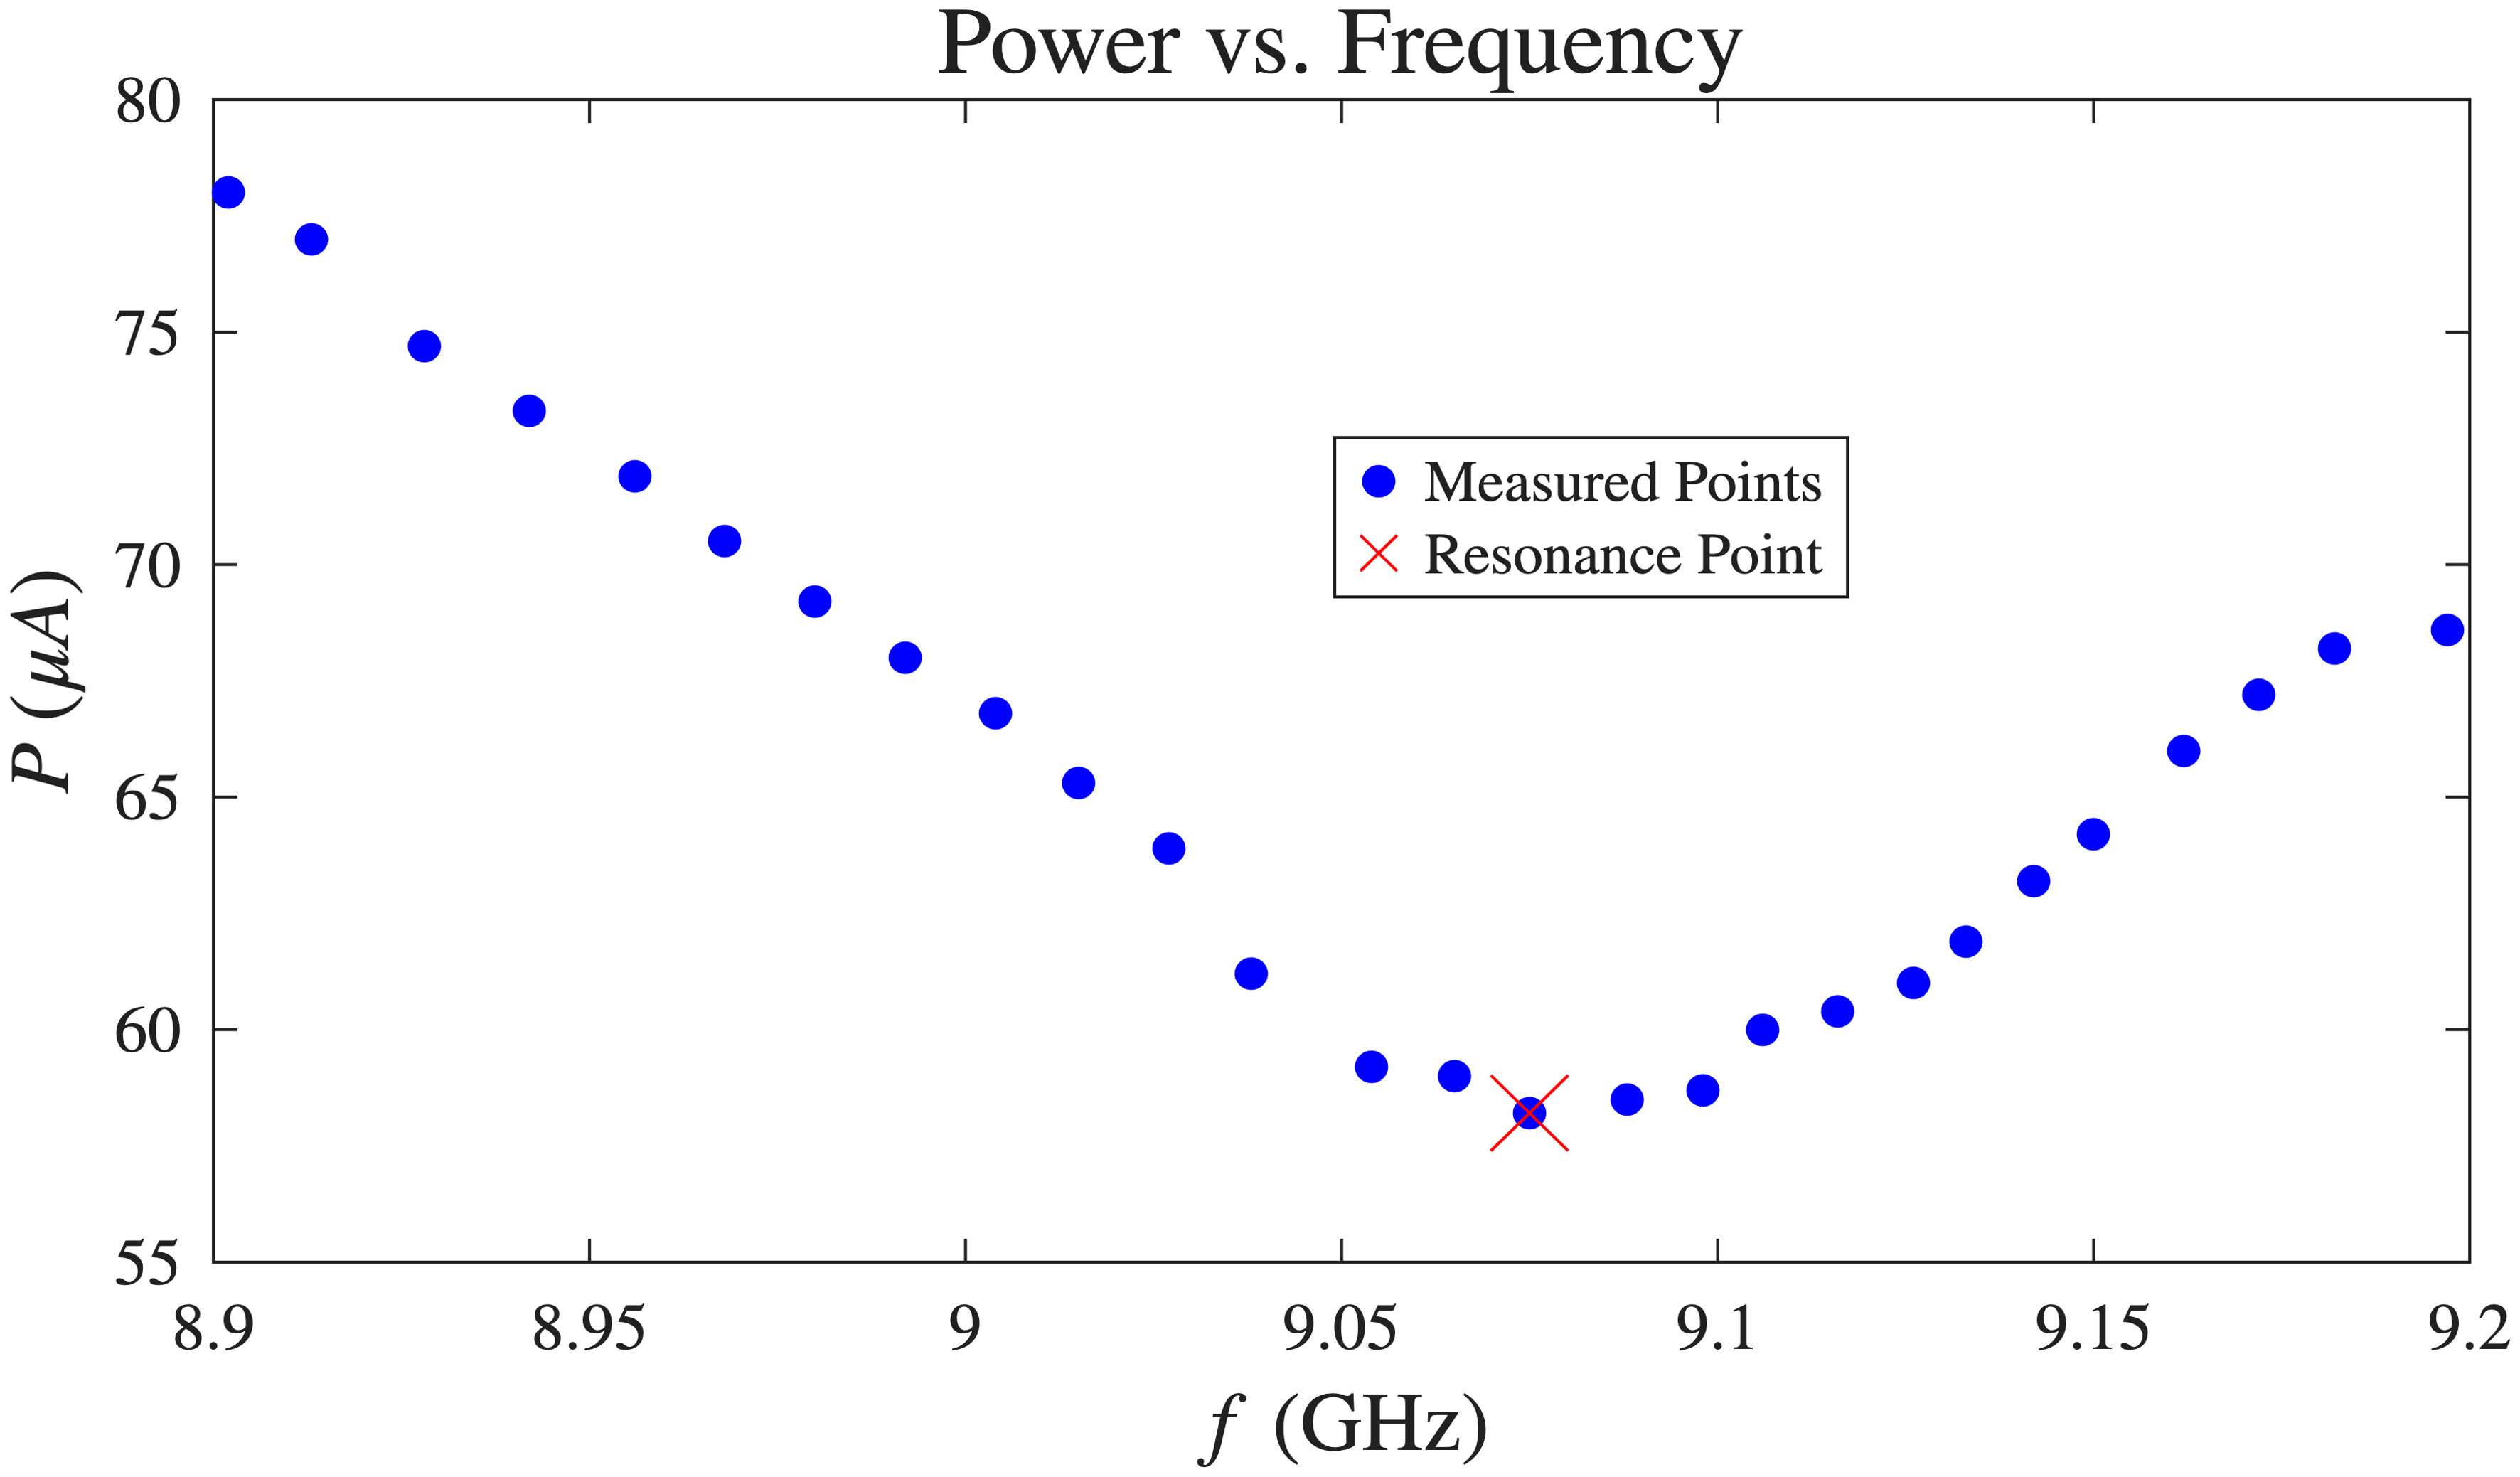
\includegraphics[width=\textwidth]{fig/fig3}
\caption{不同频率下微波输出功率}
\label{fig:Pf}
\end{subfigure}
\caption{体效应振荡器性能测量结果}
\label{fig:111}
\end{figure}


\subsubsection{体效应管 $f-U$ 曲线}

在 $10\sim13\,\text{V}$ 的电压范围内测量不同工作电压下的微波输出频率，得到 $f-U$ 曲线，如图\ref{fig:fU} 所示。

对测量数据进行线性拟合，可得到频率与电压之间的关系：


\centerline{$f = 39.53V + 8.4186 \times 10^3$}


拟合优度 $R^2 = 0.9867$，说明在该电压范围内微波频率与工作电压之间近似满足线性关系。


\subsubsection{不同频率下微波输出功率的测量}

在标准工作电压 $12.0\,\text{V}$ 条件下，在 $8.9\sim9.2\,\text{GHz}$ 的频率范围内调节微波频率，并测量晶体检波器的输出信号强度，以表征微波输出功率，测量结果如图\ref{fig:Pf} 所示。

由图可以看出，微波输出功率随频率变化呈现明显的非单调变化趋势。当频率从 $8.9\,\text{GHz}$ 增加时，功率逐渐减小，并在 $f \approx 9.075\,\text{GHz}$ 附近达到最小值；继续增大频率后，功率又重新增大，整体表现为近似 “U” 形曲线。

该最小值对应的频率可以视为系统可能的共振频率附近。在共振条件下，微波在谐振结构中的耦合或吸收增强，因此检波器测得的输出信号减小。该结果为后续谐振腔实验提供了一个共振频率的初步估计，在后续实验中将通过直接测量谐振曲线对该频率进行进一步验证。

\subsection{铁磁共振测量}

\subsubsection{无样品条件下谐振腔谐振曲线的测量}

实验所使用的矩形谐振腔参数为 $a=2.295\,\text{cm}$，$l=19.30\,\text{cm}$，模式参数 $p=8$。根据谐振腔理论公式计算可得其理论共振频率为
$f = 9.021\,\text{GHz}$。

结合前一部分实验中对微波输出功率随频率变化关系的初步观察，可以判断系统的共振频率位于该频率附近。因此在该频率附近调节微波频率，并通过调节衰减器使测量过程中 $\mu$A 表始终保持在同一量程范围内，从而减小量程变化带来的系统误差。

在共振频率附近逐点改变微波频率并记录检波器输出信号，得到谐振腔无样品时的谐振曲线，如图 \ref{fig:cavity_resonance} 所示。

\begin{figure}[h!]
    \centering
    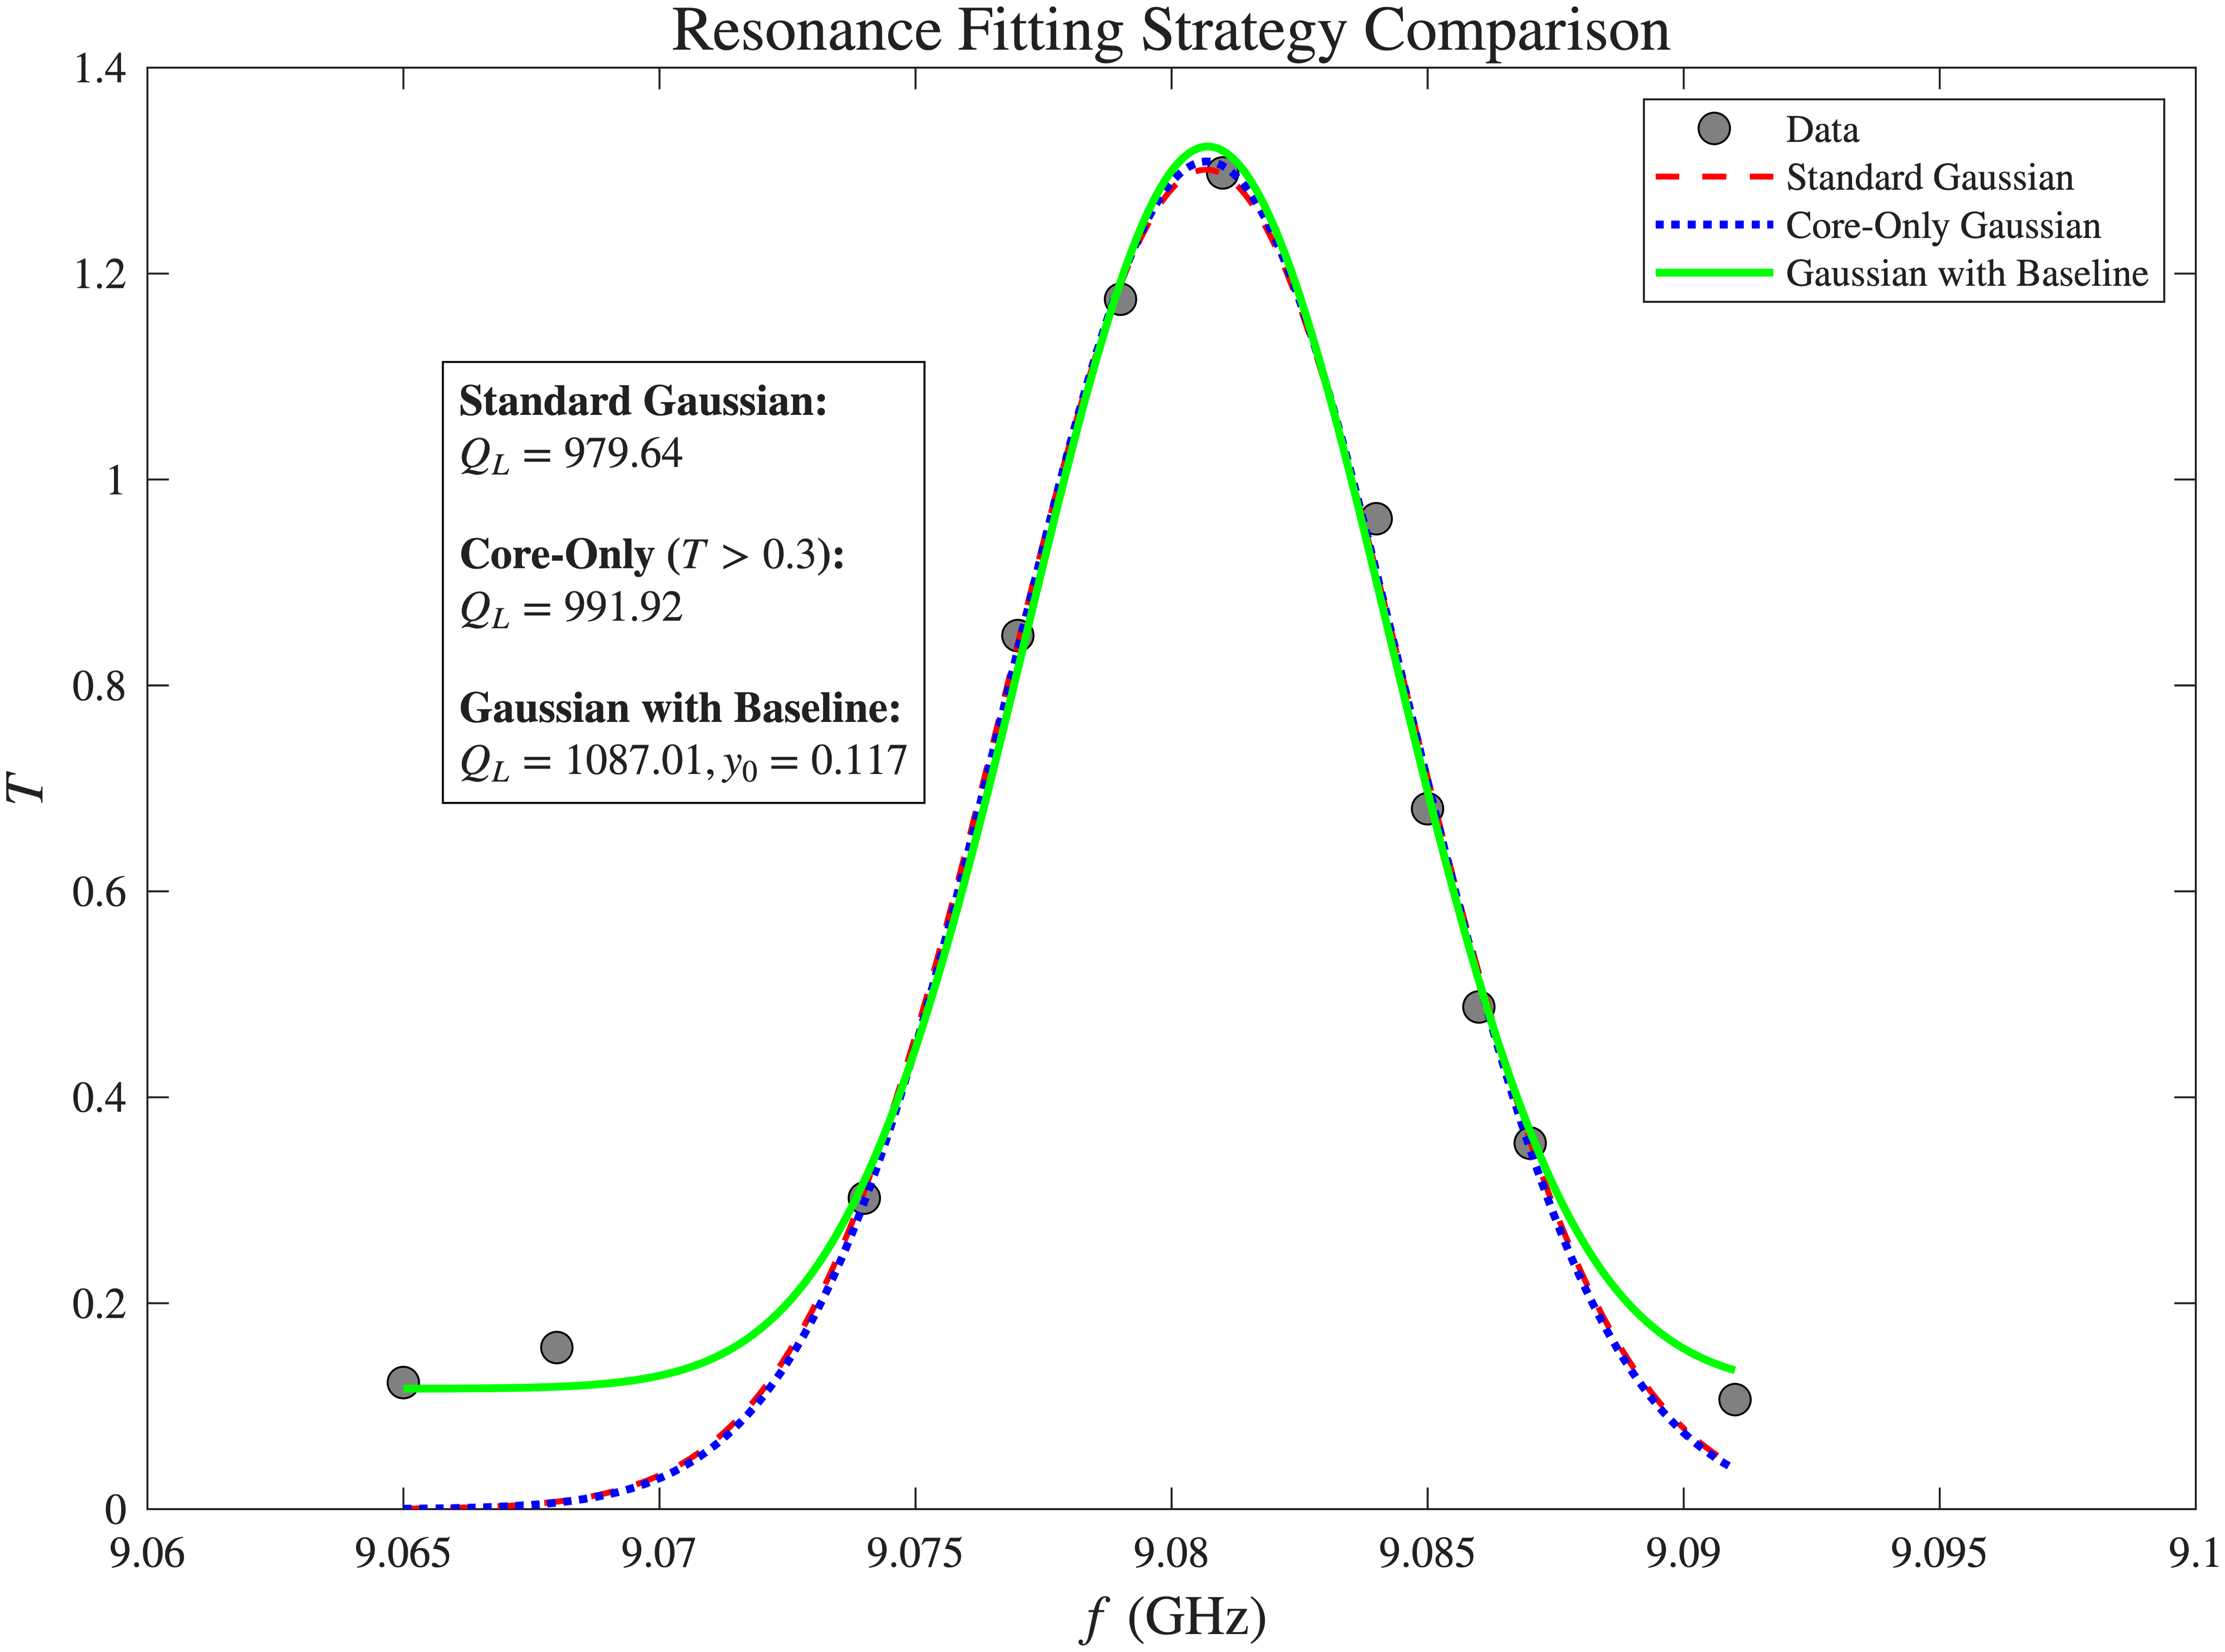
\includegraphics[width=0.8\textwidth]{fig/fig4.png}
    \caption{谐振腔无样品时的谐振曲线}
    \label{fig:cavity_resonance}
\end{figure}

从实验数据可以观察到，谐振频率两侧的数据分布存在一定的不对称性。如果直接对全部数据进行高斯函数拟合，可能会引入一定误差。因此采用三种不同的数据选取方式进行拟合比较。

第一种方法对全部数据进行拟合，记为“拟合1”(Standard Gaussian)；第二种方法仅选取共振频率附近的数据进行拟合，以减小尾部数据偏移对结果的影响，记为“拟合2”(Core-Only)；第三种方法在高斯函数上加一个基线，以降低“底噪”对结果的影响，记为“拟合3”(Gaussian with Baseline)。拟合函数选取为

\begin{equation*}
T(f)= a \exp\left(-\left(\frac{f-b}{c}\right)^2\right) + y_0
\end{equation*}

两次拟合结果分别为

\begin{align*}
\text{Standard Gaussian：}\quad a&=1.3009 \qquad b=9.0807 \qquad c=0.0056 \qquad R^2=0.9747 \\
\text{Core-Only：}\quad a&=1.3089 \qquad b=9.0807 \qquad c=0.0055 \qquad R^2=0.9952 \\
\text{Gaussian with Baseline：}\quad a&=1.2065 \qquad b=9.0807 \qquad c=0.0050 \qquad y_0 = 0.1169 \qquad R^2=0.9950
\end{align*}

由拟合参数可以得到谐振腔共振频率以及加载品质因数

\[
f_0=b \qquad 
Q_L=\frac{b}{2\sqrt{\ln2}\,c}
\]

从而得到

\begin{align*}
\text{Standard Gaussian：}\quad f_0&=9.0807\mathrm{GHz} \qquad Q_L=979.64 \\
\text{Core-Only：}\quad f_0&=9.0807\mathrm{GHz} \qquad Q_L=991.92 \\
\text{Gaussian with Baseline：}\quad f_0&=9.0807\mathrm{GHz} \qquad Q_L=1087.01
\end{align*}

\textbf{误差分析}

将实验测得的共振频率与理论值进行比较，可以得到相对误差

\[
\eta = \frac{\Delta f}{f_{0,\text{理论}}}\times100\% = 0.662\%
\]

实验结果表明测得的共振频率与理论计算值基本一致，说明实验测量具有较好的可靠性。

另一方面，不同拟合方式得到的品质因数存在一定差异。这主要是由于实验曲线在高频一侧存在轻微偏移，其原因可能与体效应振荡器输出功率随频率变化的背景趋势有关，因此会对高斯拟合结果产生一定影响。

\subsubsection{放入样品后的共振曲线定性观察}

在确定合适的微波频率后，将电磁铁工作模式设为扫场模式，并将样品置于谐振腔中，通过示波器观察输出信号与扫场信号构成的 X-Y 图像。通过调节相位、扫场幅度以及直流偏置，可以获得较为清晰的共振信号。

实验中使示波器进行往复扫描，使上升沿与下降沿对应的共振峰位置尽可能重合，从而得到较为稳定的共振曲线。随后分别改变相位、直流电流以及扫场幅度，观察共振曲线的变化规律。

实验现象总结如下：

\begin{itemize}

\item \textbf{相位变化}  
改变相位会导致两个共振峰的位置发生移动，但对峰的展宽和高度影响较小。

\item \textbf{直流电流变化}  
改变直流电流会使共振峰整体发生平移。当电流减小时，共振峰整体向左移动；电流增大时，共振峰整体向右移动，而峰宽与峰高变化不明显。

\item \textbf{扫场幅度变化}  
扫场幅度主要影响共振峰的展宽。扫场增大时峰宽减小，扫场减小时峰宽增大，而峰高基本保持不变。

\end{itemize}

在完成上述定性观察后，更换不同类型的样品并观察其共振曲线。实验发现单晶样品与多晶样品在共振曲线形状上存在明显差异，如图 \ref{fig:single_poly} 所示。

\begin{figure}[h!]
    \centering
    \begin{subfigure}{0.47\textwidth}
        \centering
        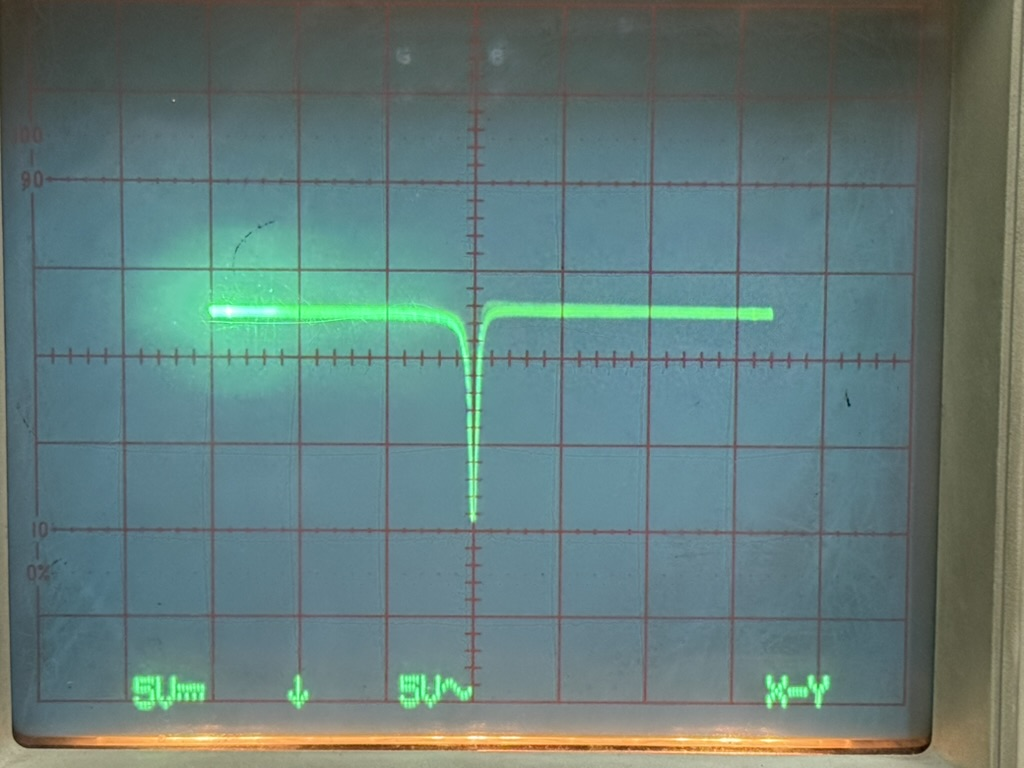
\includegraphics[width=\textwidth]{fig/fig5.jpeg}
        \caption{单晶样品的共振曲线}
    \end{subfigure}
    \hfill
    \begin{subfigure}{0.47\textwidth}
        \centering
        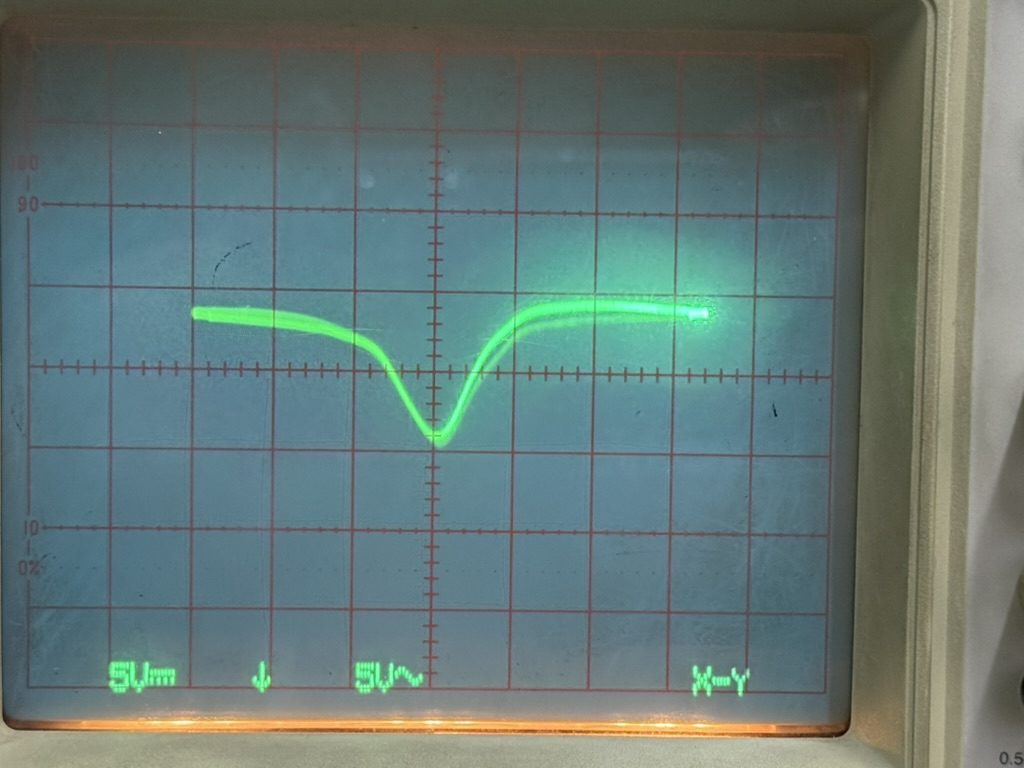
\includegraphics[width=\textwidth]{fig/fig6.jpeg}
        \caption{多晶样品的共振曲线}
    \end{subfigure}
    \caption{不同类型样品的铁磁共振曲线比较}
    \label{fig:single_poly}
\end{figure}

单晶样品中晶体取向较为一致，因此共振条件较为集中，共振线宽相对较小，曲线表现为较尖锐的吸收峰。

多晶样品由大量取向不同的晶粒组成，各晶粒的共振条件存在差异，因此整体共振信号可视为多个共振位置的叠加结果，从而表现为较宽的共振线宽以及相对平缓的曲线形状。

\subsubsection{逐点法测量共振曲线}

由于多晶样品共振线宽较大，测量过程中更容易获得完整的共振曲线，因此本实验选择多晶样品进行定量测量。

首先通过粗略调节频率确定共振的大致位置，然后在共振点附近采用较小步长进行测量，而在远离共振区域的位置适当增大步长。通过逐点改变磁场电流并记录输出信号，得到共振吸收曲线，如图 \ref{fig:mag_curve} 所示。

\begin{figure}[h!]
    \centering
    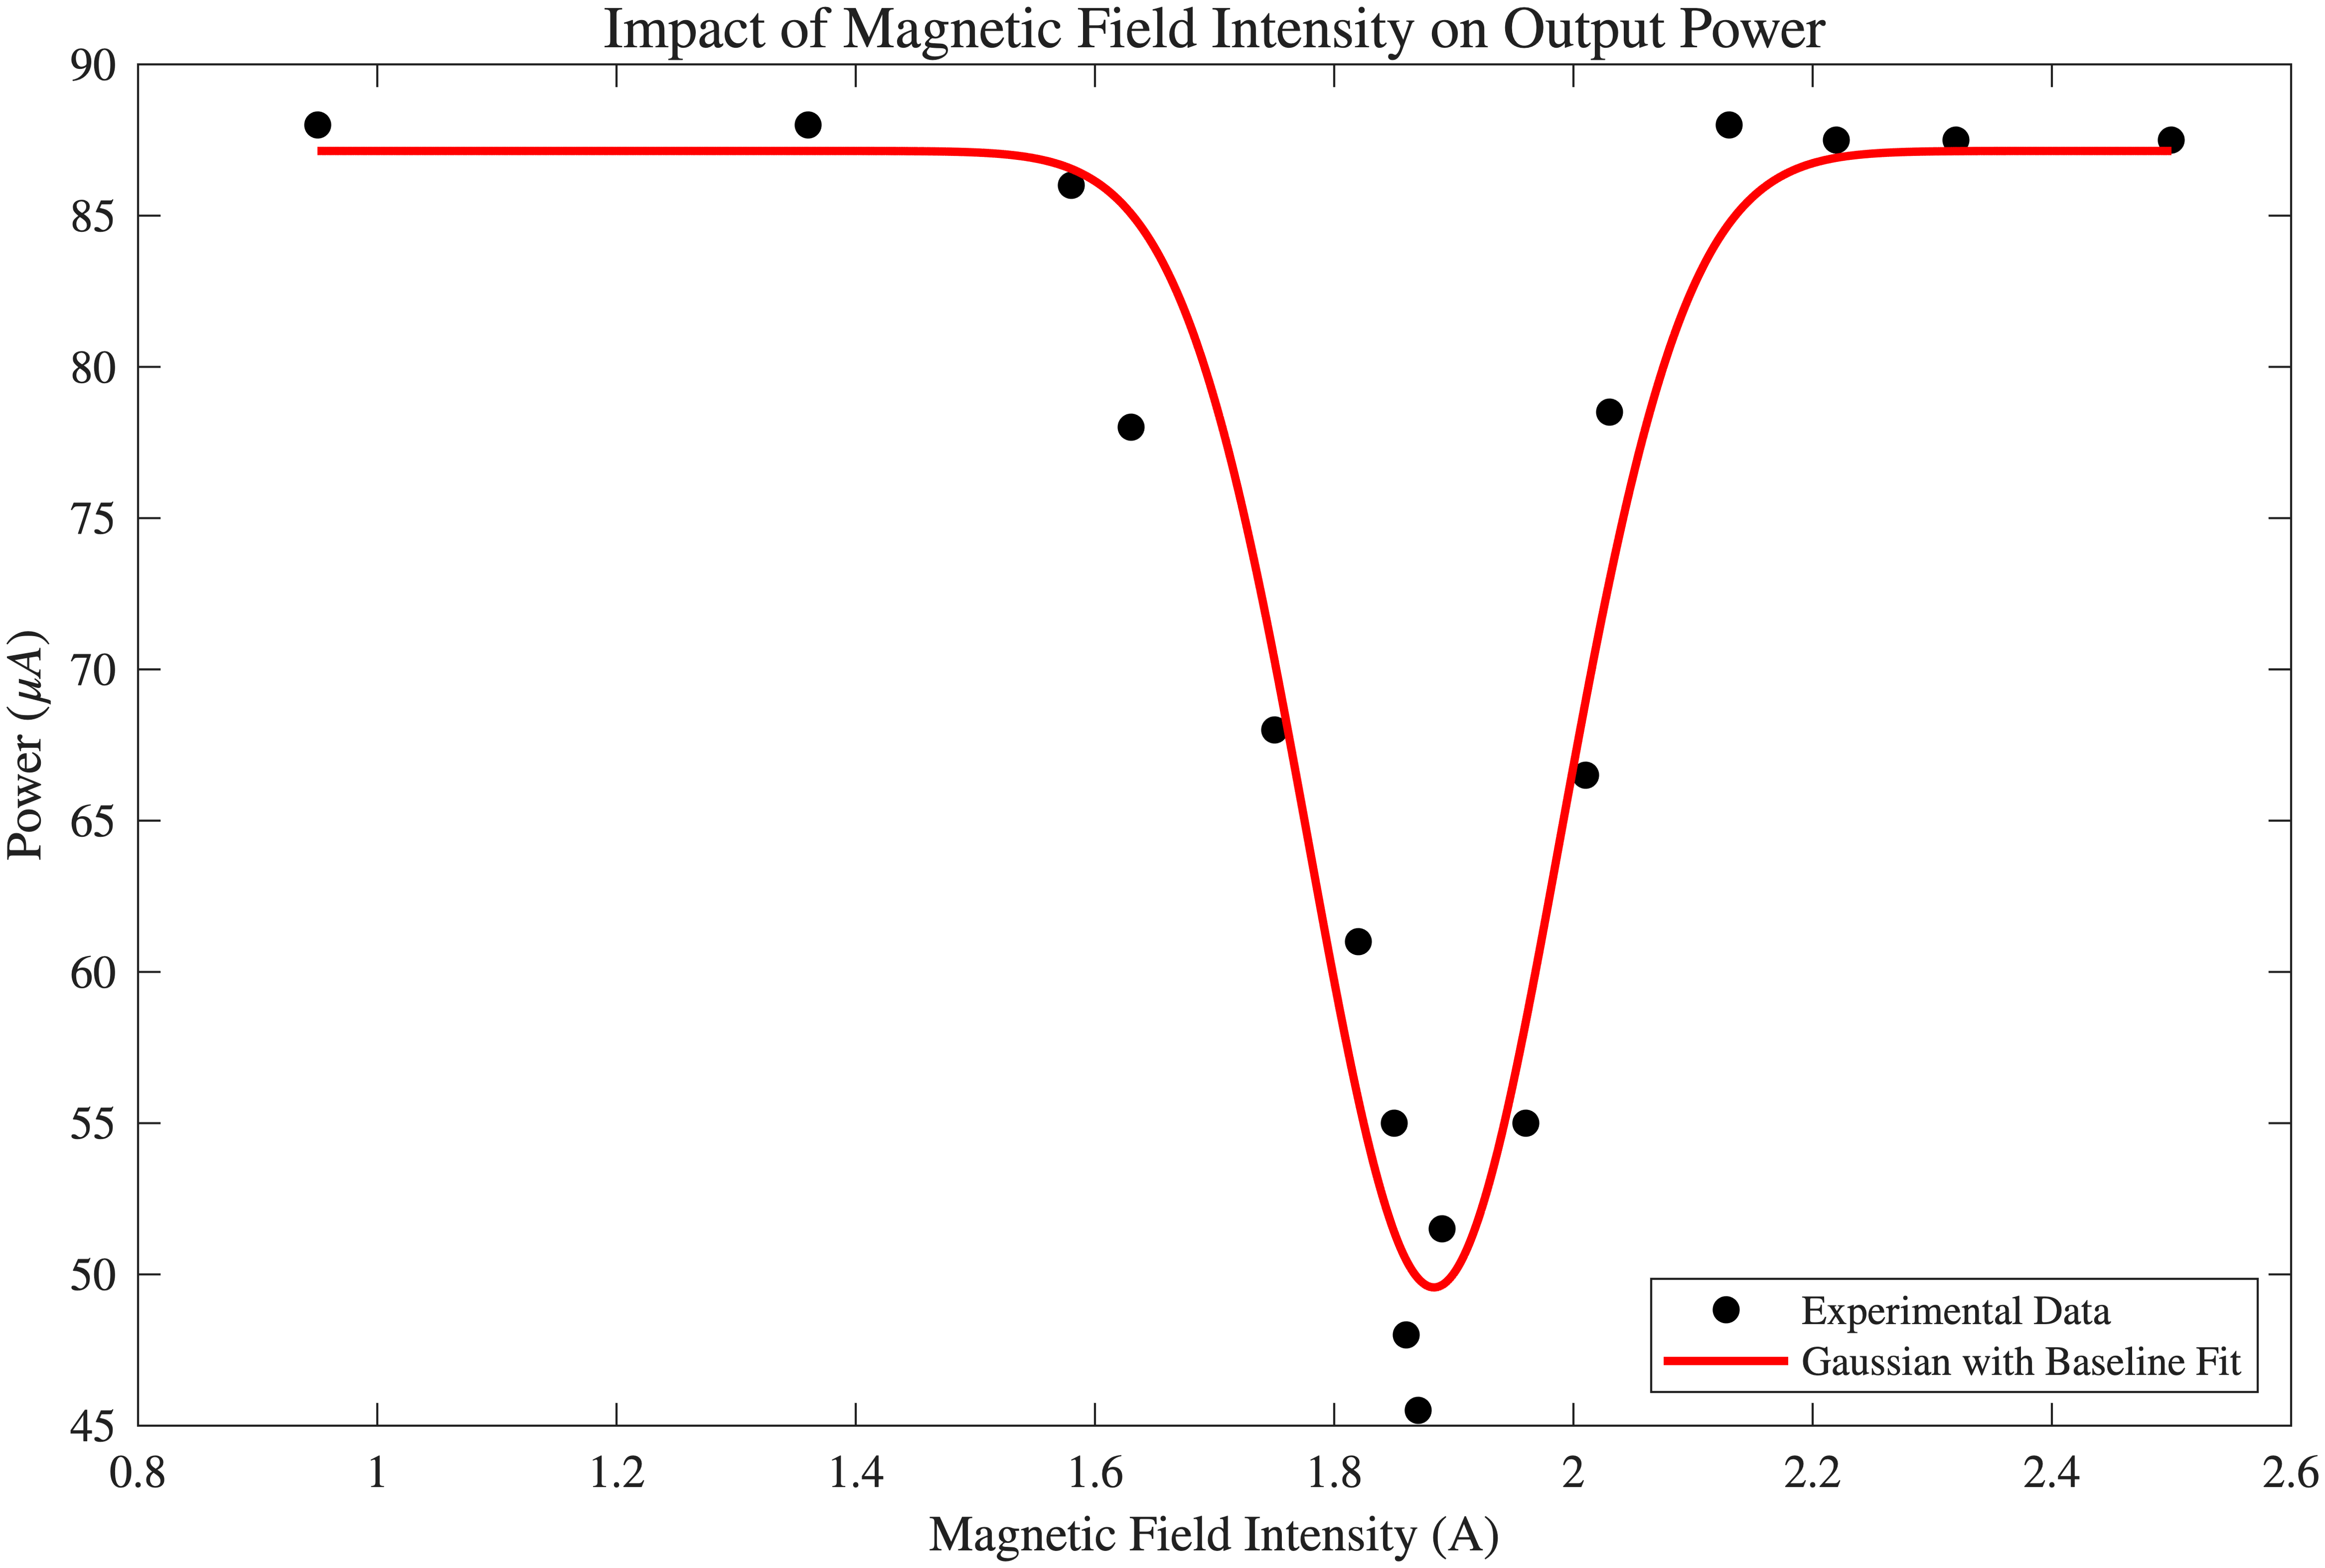
\includegraphics[width=0.9\textwidth]{fig/fig7.png}
    \caption{多晶样品的共振曲线}
    \label{fig:mag_curve}
\end{figure}

实验数据采用高斯函数进行拟合

\[
P(H)= a\exp\left(-\frac{(H-b)^2}{2c^2}\right)+d
\]

拟合参数为

\[
a=-37.5674 \qquad
b=1.8834 \mathrm{A} \qquad
c=0.1488 \qquad
d=87.1382 \mathrm{\mu A}
\]

拟合优度为

\[
R^2=0.9560
\]

从实验结果可以看到，在远离共振条件时，输出功率基本保持在较为稳定的水平；随着磁场逐渐接近某一特定范围，输出功率出现明显下降，在该区域形成一个较为明显的吸收谷。这一现象表明在该磁场条件下样品发生铁磁共振，微波能量被样品有效吸收，从而导致检测到的输出功率减小。

为了更加清晰地确定共振位置及其线形特征，对实验数据进行了函数拟合。考虑到实验背景信号可能存在一定基线偏移，并且共振吸收曲线在统计意义上近似呈现高斯分布，因此采用包含基线项的高斯函数对数据进行拟合。拟合结果表明实验数据能够较好地被该模型描述，共振位置对应于输出功率最低点附近。

需要指出的是，由于多晶样品由大量取向不同的晶粒组成，各晶粒的有效共振条件并不完全相同，因此整体观测到的共振信号实际上是多个共振贡献的叠加结果。这种取向分布会导致共振曲线出现一定程度的展宽，使得实验得到的吸收谷相对于单晶样品更加宽缓。该特征也与铁磁共振实验中多晶材料的典型表现相一致。

\subsubsection{高斯计测量磁场 $I-B$ 标定曲线}

撤去谐振腔后，将高斯计探头放置在电磁铁中心位置，对电磁铁磁场进行标定测量。实验得到磁场与电流之间的关系曲线，如图 \ref{fig:IB_curve} 所示。

\begin{figure}[h!]
    \centering
    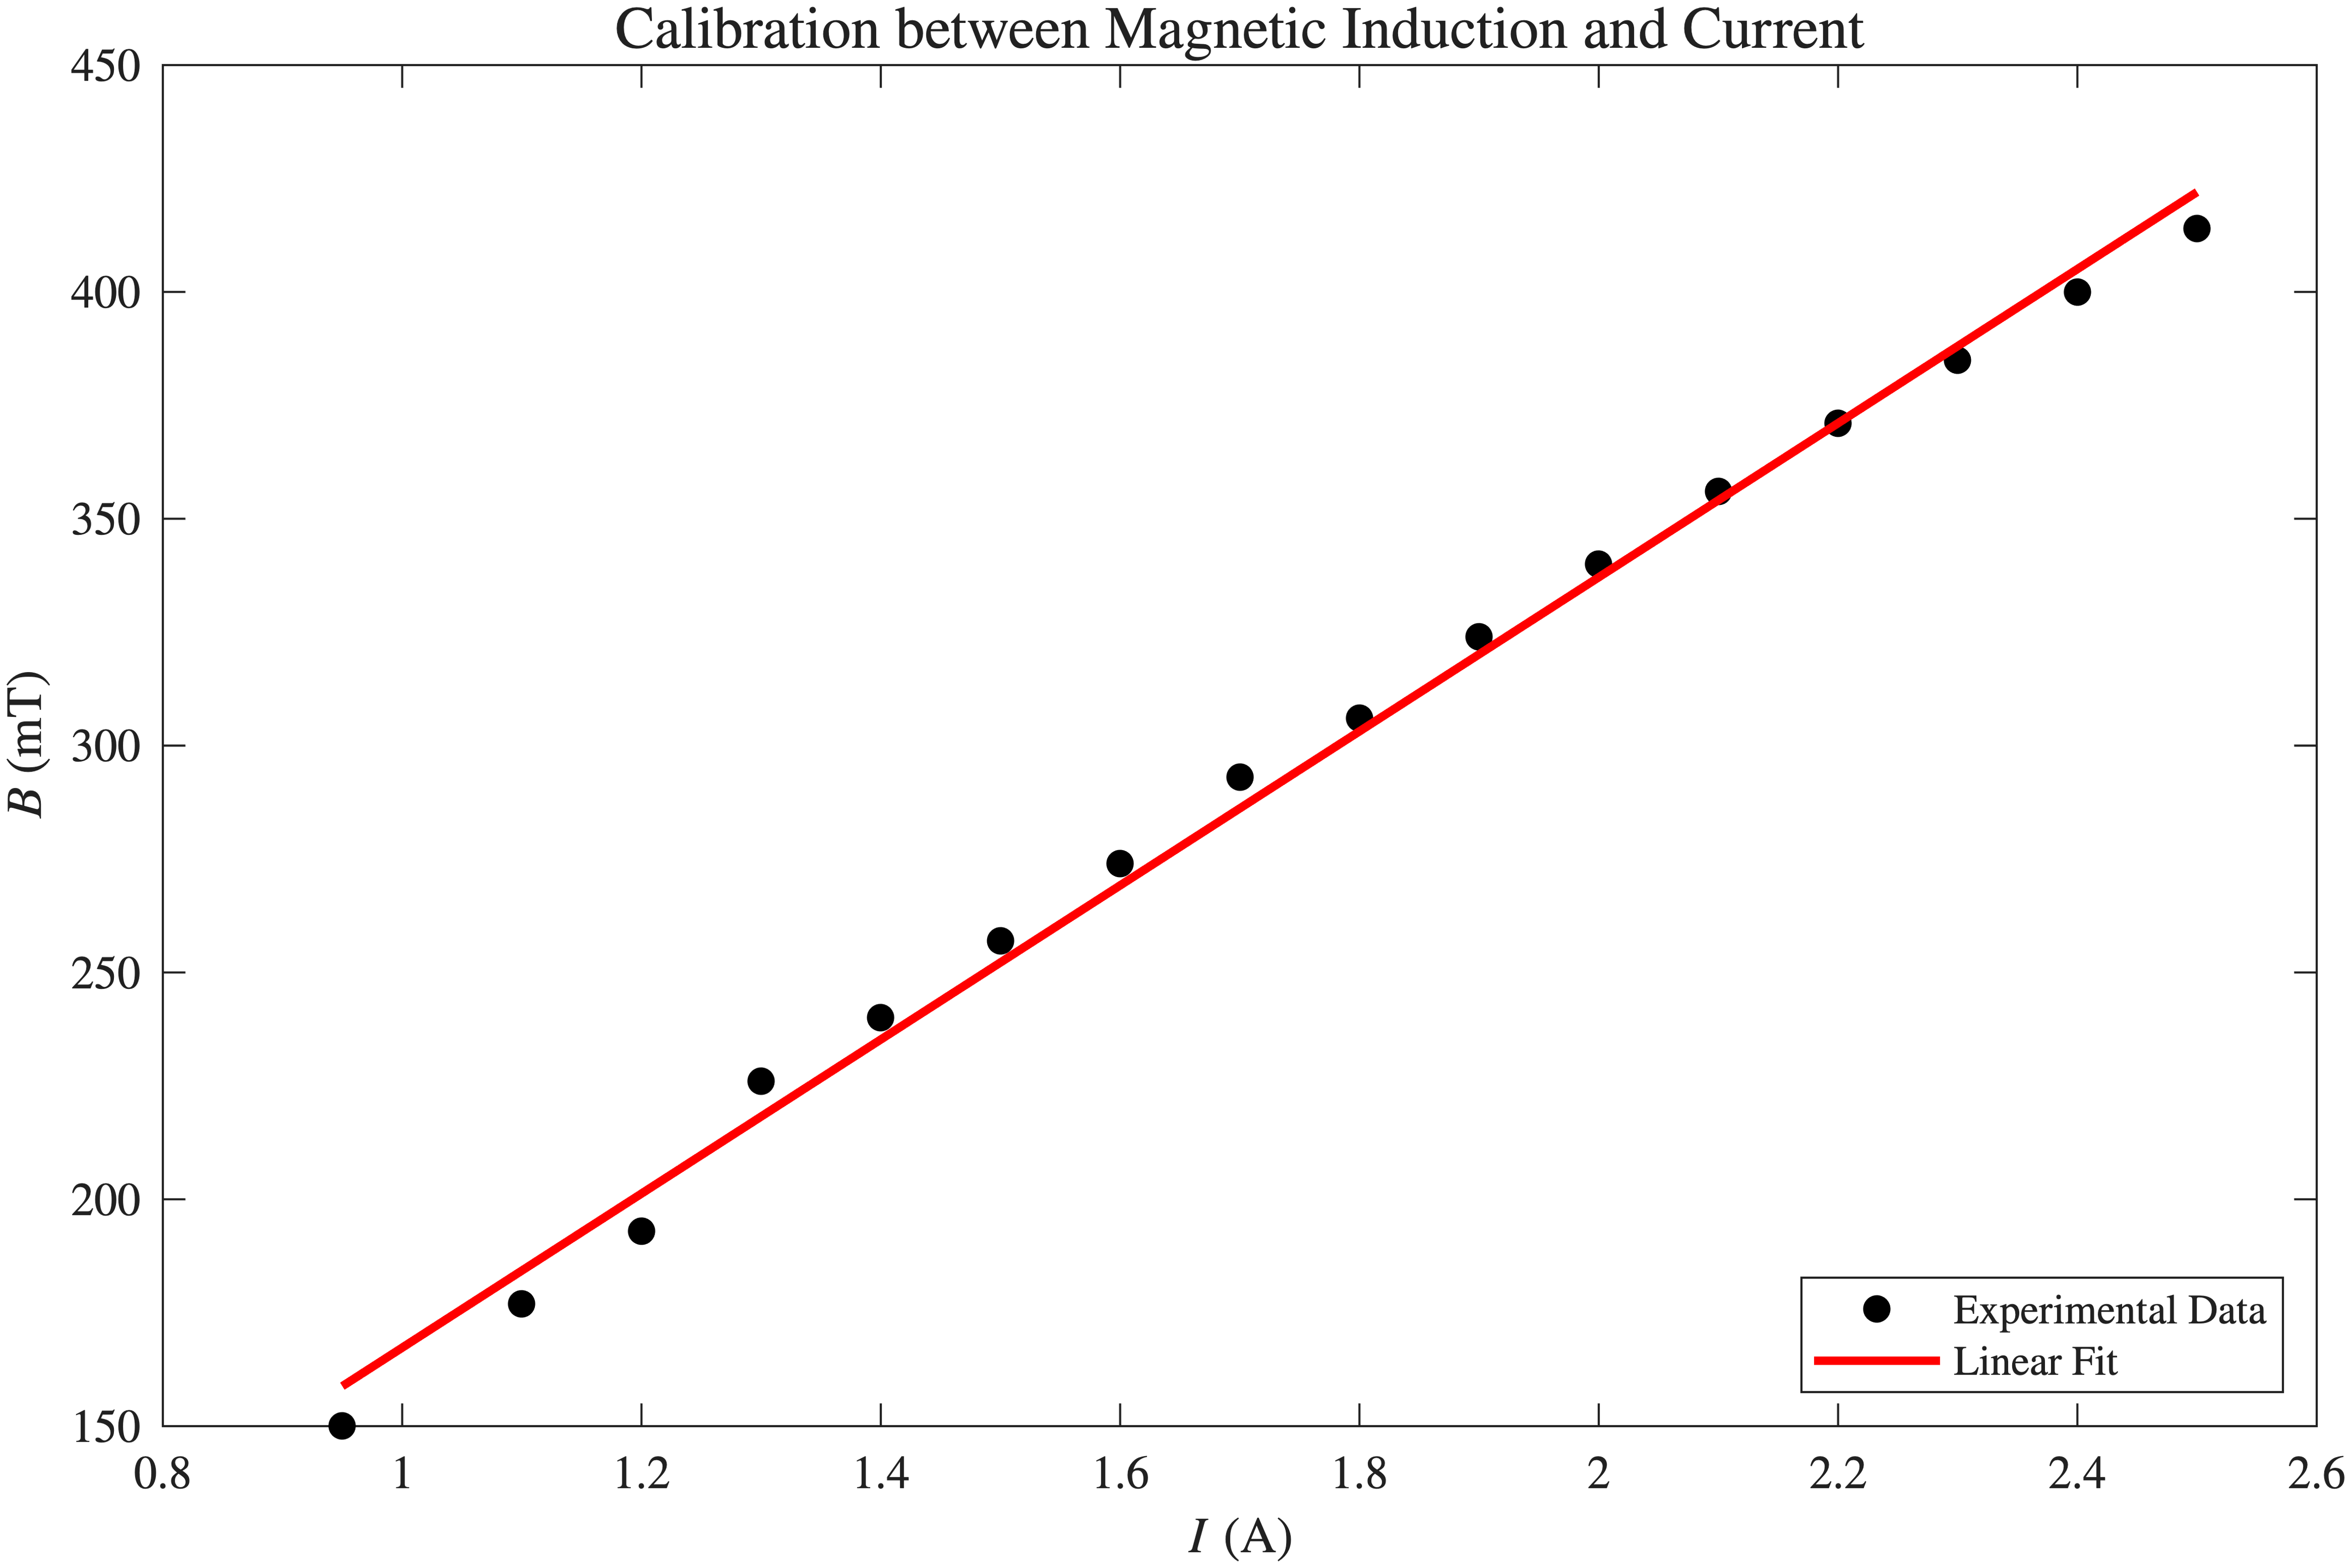
\includegraphics[width=0.75\textwidth]{fig/fig8.png}
    \caption{电磁铁的 $I-B$ 标定曲线}
    \label{fig:IB_curve}
\end{figure}

对实验数据进行线性拟合，可以得到磁场与电流之间的关系式

\begin{equation}
B = kI + B_0
\end{equation}

其中

\[
k=169.8153\mathrm{mT/A} \qquad B_0=-2.5211 \mathrm{mT}
\]

拟合优度为

\[
R^2=0.9950
\]

\subsubsection{旋磁比、朗德因子与弛豫时间计算}

根据共振吸收曲线可以计算共振线宽。利用半高宽关系式

\[
P_{1/2} = \frac{2 P_r P_0}{P_r + P_0}
\]

结合拟合参数可以得到电流尺度下的共振线宽

\[
\Delta I = 0.3967\mathrm{A}
\]

再结合磁场标定关系式，可以得到磁场尺度下的线宽

\[
\Delta B = k\Delta I = 67.36\mathrm{mT}
\]

共振磁场为

\[
B_0 = kI_{\text{res}} + B_0 = 317.31 \mathrm{mT}
\]

进一步可以计算旋磁比

\[
\gamma = \frac{\omega}{B_0} = \frac{2\pi f_0}{B_0} = 1.78\times 10^{11} \mathrm{rad/(s\cdot T)}
\]

从而得到朗德因子

\[
g = \frac{2m\gamma}{e} = 2.045
\]

弛豫时间为

\[
\tau = \frac{2}{\gamma\Delta B} = 0.165\mathrm{ns}
\]
    \section{总结}

    本实验利用微波体效应振荡器产生稳定的微波信号，并结合传输式谐振腔对铁氧体样品进行了铁磁共振研究。通过对磁场的调节以及共振信号的观测，成功获得了单晶和多晶样品的磁共振曲线，并对其物理特性进行了分析。

在实验过程中，首先测量了体效应振荡管的工作特性曲线。实验结果表明，在适当的偏置电压范围内振荡器能够产生稳定的微波输出，为后续的共振实验提供了可靠的微波源。随后通过谐振腔调谐确定了合适的工作频率，使系统能够在最佳耦合条件下进行磁共振测量。

在样品测量部分，通过扫场法以及逐点法对样品的共振信号进行了观测。实验中可以明显看到，当外加磁场满足铁磁共振条件时，谐振腔中的微波能量被样品吸收，从而在输出信号中形成明显的吸收谷。对共振曲线进行分析后发现，单晶样品的共振峰较为尖锐、线宽较小，而多晶样品的共振曲线则明显展宽。这一差异主要来源于样品内部晶粒取向的不同：单晶样品的晶格取向较为一致，而多晶材料由大量取向随机的晶粒组成，因此整体共振信号表现为多个共振条件的叠加。

在定量分析方面，通过逐点法测量获得多晶样品的共振曲线，并利用包含基线项的高斯函数对实验数据进行了拟合，从而确定了共振位置以及线宽参数。在此基础上进一步计算得到样品的朗德因子和弛豫时间，其结果分别为
$g = 2.045$，
$\tau = 0.165\mathrm{ns}$。
实验得到的结果与铁磁共振理论的预期量级一致，表明实验方法能够较好地反映样品的磁动力学特性。

总体而言，本实验通过微波谐振腔技术成功实现了对铁氧体材料铁磁共振现象的观测，并通过共振曲线分析获得了材料的重要物理参数。实验不仅加深了对微波技术和磁共振原理的理解，也进一步体现了材料微观结构对磁动力学行为的重要影响。
    \begin{thebibliography}{99}
        \bibitem{1}
        北京师范大学物理实验教学中心. 近代物理实验讲义一 (2019)
    \end{thebibliography}

    
\end{document}